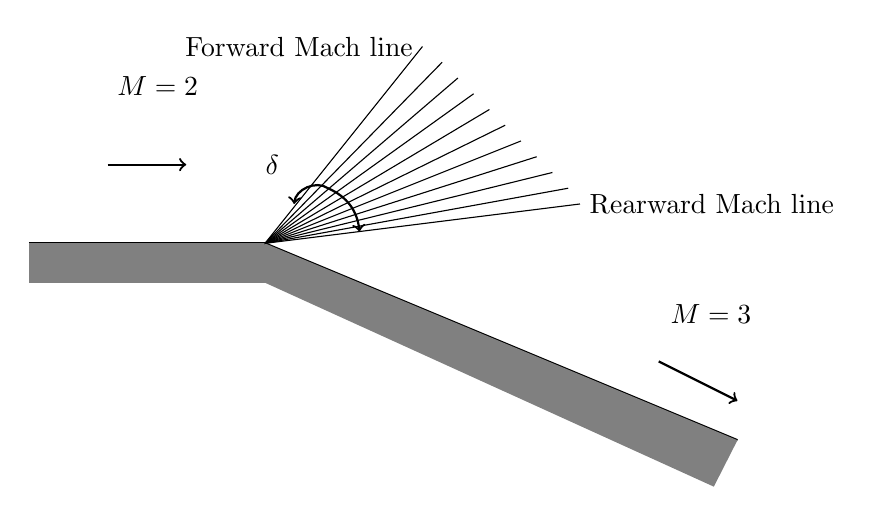
\begin{tikzpicture}
    


    \draw[thick] (-1,5.5) -- (2,5.5);
    \fill[gray!] (-1,5) -- (-1,5.5) -- (2,5.5) -- (2,5) -- cycle;
    \draw[thick] (2,5.5) -- (8,3);
    \fill[gray!] (2,5.5) -- (8,3) -- (7.7,2.41) -- (2,5) -- cycle;
    % Add other related components or labels as needed
    \node[right] at (0,7.5) {$M=2$};
    \draw[->, thick] (0,6.5) -- (1,6.5);

    \draw (2,5.5) -- (4,8)  node[left] {Forward Mach line};
    \draw (2,5.5) -- (6,6)  node[right] {Rearward Mach line};
    \draw (2,5.5) -- (5.85,6.2) ;
    \draw (2,5.5) -- (5.65,6.4) ;
\draw (2,5.5) -- (5.45,6.6) ;
\draw (2,5.5) -- (5.25,6.8) ;
\draw (2,5.5) -- (5.05,7) ;
\draw (2,5.5) -- (4.85,7.2) ;
\draw (2,5.5) -- (4.65,7.4) ;
\draw (2,5.5) -- (4.45,7.6) ;
\draw (2,5.5) -- (4.25,7.8) ;


 \draw[<->, thick] (2.37,6.0) to[bend left=60] (2.8,6.2) to[bend left=30] (3.2,5.65);


    \node[left] at (8.3,4.6) {$M=3$};
    \node[left] at (2.3,6.5) {$\delta$};
     \draw[->, thick] (7,4) -- (8,3.5);
\end{tikzpicture}